

\section{Multi-episodic Perceived Quality}\label{chap:state-of-the-art}
%\begin{chapter-abstract}
%%NOTE: This chapter might be too small, consider merging with previous chapter.
%Here I present the state of the art on multi\-/episodic QoE \citet{duncanson_average_1969}, and \citet{moller_single-call_2011}.
%It is important to state again the research question (How do subjects integrate low episodic quality into an overall experience?) for this domain and introduce methodologies.
%Major point here is the research method (task-driven, defined usage behavior, limited freedom in usage behavior).
%At the end of this chapter I must have made clear what methodologies are used and also made clear what their respective target is.
%\end{chapter-abstract}

%\cite{staelens_assessing_2009}
%\cite{schatz_vienna_2011}, 3 Weeks!
Services are in general used on a regular basis by a user~\citep[\cf{}][]{geerts_linking_2010}.
The experiences of a usage episode lead to a perceived quality in the user of this very episode.
The definition of \emph{usage episode} in the context of multi\-/episodic perceived quality is derived from the concept of episodic memory (\cf{} \autoref{chap:03}), focusing on usage of telecommunication systems.
In addition, goal achievement as a requirement is added, following the concepts of utility and expected utility by \citet{kahneman_experienced_2000}.

\begin{definition}[Usage Episode]\label{def:episode}
A usage episode is a distinct, meaningful, and self-contained interaction by a user with a service or system to achieve his goal(s).
\end{definition}
Multi\-/episodic perceived quality results from a \emph{formation process}, combining prior experiences and their perceived quality.
In fact, prior experiences can affect the \emph{quality formation process} and thus influence the perceived quality of later experiences. 
Also, a user's behavior towards a service might change due to perceived quality affecting usage frequency, task-solving strategies, or even lead to abandoning the service completely.
Multi\-/episodic perceived quality is thus the result of a sequential process.
Here, the order of usage episodes and their individual experiences affect the final judgment.
Investigations on multi\-/episodic perceived quality can therefore only be undertaken in experiments adhering to a between-subject design.
Here, every participant is only exposed to a single \emph{multi\-/episodic} condition.\footnote{A within-subject design might applicable for the investigation of multi\-/episodic perceived quality if it can be ensured that the presentation order of different \emph{multi\-/episodic} conditions does not affect the multi\-/episodic judgment for each condition.} 
In the following, the word \emph{episode} is used as a synonym of usage episode.

In the field of \ac{QoE}, multi\-/episodic perceived quality has so far only received limited attention.
For practical use, it is often sufficient to understand the relationship between different performance parameters and the impact on perceived quality in a time frame ranging from seconds up to some minutes.
Thus, an influence of time, tasks, and other factors on perceived quality is often neglected.
However, understanding the formation process of multi\-/episodic perceived quality enables, for example, a service provider to serve a better service for his users.

\subsection{Excursus: Multi-episodic usage in \acs{UX}}
Effects of multi\-/episodic usage while focusing on changes in user behavior have been evaluated in \ac{UX}.
\ac{QoE} and \ac{UX} conceptually overlap as both focus on experiences in general and experiences with technology \citep[\cf{}][]{wechsung_quality_2014}.
\ac{UX}, stemming from usability, focuses on the interaction with technology and how interactions affect usage as well as emotions towards used technology.\footnote{For a longer discussion on similarities and difference between \ac{QoE} and \ac{UX} see \citet{wechsung_quality_2014} and also \citet{hassenzahl_user_2008}.}
Multi\-/episodic evaluation is an important aspect of \ac{UX}, because user behavior towards technology changes as a user learns how to use the technology and which tasks are well-suited to its use.
The multi\-/episodic concept is described by \citet[p.\,8]{roto_user_2011}.
However, they failed to put it into context with prior work and omitted their definitions.

Two major experiments that assessed the use of products over a longer usage period have been conducted.
\citet{karapanos_user_2009} investigated in one experiment how the expectations and behavior towards a new smart phone change in a usage period of four weeks. % with 6~subjects
This is extended by \citet{kujala_ux_2011} with the \emph{\ac{UX} curve} method.
Here, a participant evaluates his experiences with a product or service in retrospect.
The participant draws a line reflecting how his satisfaction changed over time and annotates the vertices with the reasons for the changes.
This also includes recalled adaptations of usage behavior.
Using this method, one experiment was conducted, evaluating the changes of satisfaction and user behavior with a new smart phone over a usage period of one year.
The experiments of \citet{karapanos_user_2009} and \citet{kujala_ux_2011} showed that the usage and emotions towards the product under investigation change over time.
In the beginning, interactions are more playful and exploratory, but over time becoming more task-oriented and productive.

Although multi\-/episodic integration is not a key aspect for \ac{UX}, it is an important aspect especially regarding the adaptation of new products and new services.

\subsection{Average Perceived Quality \citep{duncanson_average_1969}}
Initial work in the direction of multi\-/episodic perceived quality for telecommunication services was performed by \citet{duncanson_average_1969}.
Duncanson asked regular users of an oversea speech telephony service about their experience with the said service.
He investigated if there is a difference between \emph{a)} the \emph{perceived quality of a just finished call} with average performance and \emph{b)} the \emph{assumed quality} of a call with average performance.
For this experiment, Duncanson used a 4\=/point \ac{ACR} scale.\footnote{\citet{duncanson_average_1969} applied a 4\=/point \ac{ACR} scale with the labels excellent (4), good (3), fair (2), and poor (1).} % and \emph{Thurstone's Law of Categorical Judgment}.
It could be shown that judgments for case a) yield a higher score than for case b).
Duncanson concludes ``that ratings of single, recent telephone calls yield results different from ratings of subjectively averaged, past telephone calls of the same type'' \citep[][p.\,116]{duncanson_average_1969}.

Although Duncanson studied episodic perceived quality and assumed quality of a usage episode with average performance, this experiment revealed an important aspect of multi\-/episodic perceived quality.
The results indicate that the formation process of the assessed episodic perceived quality leads to a lower judgment than expected.
This suggests that the formation process does not equally weight all prior experiences with said service, but rather focuses on experiences with low performance.

\subsection{Assessment of Multi-episodic Perceived Quality}
Prior work in the direction of multi\-/episodic evaluation focuses on use, experience, and perception of a service or product under realistic conditions.
This is true for \ac{UX} as well as as for initial work on multi\-/episodic perceived quality \citep[\ie,][]{moller_single-call_2011}.

In the following section, first aspects are presented which are known to affect perceived quality and are thus important to consider for multi\-/episodic assessment.
Subsequently, the two potential assessment methods for multi\-/episodic perceived quality are presented. 

\paragraph*{Aspects}
Perceived quality for short stimuli as well as complete usage episodes is investigated by exposing multiple participants to the same stimulus or very similar stimuli and assessing the resulting perceived quality. %\citep[][p.\,11]{blauert_spatial_1996}.
The calculation of a \ac{MOS}, independent of the type of judgment or scale, results in the description of the \emph{average perceived quality}.
%The \ac{MOS} is in general assumed to reflect the perceived quality judgment of the \emph{average participant}.
With regard to multi\-/episodic perceived quality and also perceived quality in general, a \ac{MOS} can only be calculated with judgments that result from the same condition or very similar conditions.
In fact, this implicitly assumes that effects/biases are similarly for different participants with regard to the formation process of multi\-/perceived quality, \ie, the same effects with a similar characteristic occur for each participant.
In experiments on perceived quality, this assumption of \emph{temporal consistency} is in general neglected, as the time frames under investigation are rather small, \ie, usually in the range of seconds up to some minutes.
For the investigation of multi\-/episodic perceived quality, this must be taken into account as a potential confounding factor.
In fact, it is not yet known if the formation process is \emph{universal} or affected by differences between individuals.
In the following, factors are discussed that might affect multi\-/episodic perceived quality and thus should be kept constant to apply a \ac{MOS} evaluation.

%\subparagraph*{Prior Knowledge and Expectations}
Perceived quality is influenced by \emph{prior knowledge} about the service under consideration (\cf{} \autoref{related:perceivedQuality}).
This includes knowledge about the specific service and also about the type of service in general.
For example, information on the reliability of telephony services as well as knowledge about potential degradations may set expectations.
Also, promises about the performance by a service provider are considered as knowledge, \eg, performance promises about a service in an advertisement.
The availability of such information might affect expectations, attribution of degradations, and \emph{assumed quality}.
Therefore, this might affect the formation process of multi\-/episodic perceived quality.
%This is for example expressed in the \emph{E-Model} by the \emph{advantage factor} \citep{itu-t_g.107:_2015} that expresses a favorable judgment due to expected difficulty of service provision, \eg, use of a mobile phone in a remote area.

%\subparagraph*{Task, Importance and Solving Strategies}
The quality formation process is also affected by the \emph{task}, its \emph{importance}, and the \emph{task-solving strategy}.
Depending on the actual tasks, some degradations might not even be noticeable.
For example, high delay in a telephone conversation with rare turn-taking will result in a better perceived quality than in a conversation requiring more turn-taking \citep[\eg,][]{egger_it_2010, schoenenberg_quality_2015}.
Degradations might also suggest an adaptation of the task-solving strategy, \eg, reduced turn-taking due to high delay in a telephone conversation \citep[][]{schoenenberg_quality_2015}.
Also, the task-solving strategy might be adjusted over multiple usage episodes with the result that task-solving becomes more efficient.
In such a case, latter episodes will require less time and thus possibly affect the multi\-/episodic quality formation process.
Also, the importance of a task might affect the multi\-/episodic quality formation process.
A higher importance of a task can increase the likelihood of memorizing and recalling information about this specific usage episode.
This task and its episode might thus have a higher impact on multi\-/episodic perceived quality.
For example, an interviewee in a telephone job interview is likely to recall this specific episode and describe his perceived quality in difference to a common call with a friend.
Therefore, tasks, as well as the task-solving strategies and their importance, should be kept constant to avoid an undesired impact, \ie, not explainable, on multi\-/episodic perceived quality.
In addition, tasks that yield a comparable task-solving duration should be selected.

%\subparagraph*{Usage Pattern}
In addition to prior knowledge and tasks, the actual \emph{usage pattern} might also affect multi\-/episodic judgments.
A usage pattern describes when, for what, and how a service is used.
This includes how often a user is exposed to the service's performance and thus new experiences affecting the perceived quality are acquired.
A usage pattern can be regular with a defined frequency but also irregular.
In fact, different usage patterns might result in differences of multi\-/episodic judgments.
This might be due to differences in memorization, but also due to decay of memorized information.
Besides the usage pattern, the experienced performance  seems to be of greater importance.
In terms of multi\-/episodic perceived quality, this refers to the performance and its variation of all individual episodes.
%In fact, if the experienced performance as well as the usage pattern are identical or similar enough, multi\-/episodic judgments of different participants allow to derive a \ac{MOS}.

All these aspects might affect the formation process of multi\-/episodic perceived quality and thus might lead to different observable effects.
However, so far, the potential impact of these aspects on multi\-/episodic judgments is not yet known.

\paragraph{Assessment Methods}
Multi\-/episodic perceived quality can be investigated using two diametric methods which differ in the behavioral freedom of users.
On the one hand, users are allowed to interact freely with the service under investigation.
In this setting, each user can decide individually when, how, how often, and for which tasks to use this service, \ie, the individual user behavior is not limited.
On the other hand, a similar user behavior can be enforced by defining when, how, and for which tasks the service should be used.
In the following, both methods are presented in detail, and the implications are discussed.

\subparagraph*{Free-use method}
Multi\-/episodic perceived quality can be investigated by observing the interactions of a user with a service without restricting his usage behavior.
Here, users are free to select when and how to use a service, to abandon it, and also to acquire new information about it.
This approach has for example been taken by \citet{duncanson_average_1969}.
In fact, this allows the observation of \emph{real} users of a \emph{real} service.
In such a case, information about a user's usage pattern, tasks, goals, expectations, and prior knowledge is often hard to acquire.
This lack of information might be overcome by sampling a large number of users.
%Another option to reduce the impact of this lack is to gather self-reported measures of users, or complement it with behavioral data (\eg, churn, likelihood to re-buy, monetization).
Allowing users to decide when and how a service is used enables the investigation of service usage in an ecologically valid situation, \ie, how  users would behave in their current situations.
This method offers ecological validity, but limits reproducibility.

\subparagraph*{Defined-use method}\label{method:definedUse}
Limiting the user's freedom by defining when and how to interact with a service allows to present the same condition to multiple participants.
For multi\-/episodic perceived quality, this requires the definition of the usage pattern including task and performance for each usage episode.
This ensures that all participants are exposed in a similar manner to the service.
A task can be artificial, \ie, a participant does not necessarily engage in such a task on his own, and should lead to a similar task-solving strategy.
For telecommunication services, this could be a telephone call with defined content or listening to a recorded telephone call. %Friedemann: zweiter Teil weg

To limit an influence of prior experiences and information about a service, it must be ensured that users have similar knowledge about the service and similar prior exposure to the service.
This can be achieved by a careful selection of users or by creating a \emph{new service}.
In fact, a new service only prevents the existence of prior experiences with this service, but cannot avoid the impact of prior knowledge, for example, about typical degradations for such a service type in general.
This assessment method is here denoted as defined-use method.
Here, the usage pattern as well as the task and the performance per usage episode are defined.
Such a set is denoted as \emph{multi\-/episodic condition}.
Exposing multiple participants to the same multi\-/episodic condition allows to derive a \ac{MOS}.
The impact of varying performance on multi\-/episodic perceived quality can then be investigated by changing only the performance between otherwise identical conditions.
This method limits ecological validity, enabling however in the process reproducibility.

\subparagraph*{Discussion}
Both assessment methods are diametrically opposed. 
Free-use allows studying multi\-/episodic perceived quality with existing users by observing their interaction with said service and optionally gathering direct feedback.
This non-intrusive method is, however, in general limited by the obtainable information about a user.
In addition, the performance of a \emph{real} service can hardly be controlled and the desired degradations might not occur reliably enough.
In fact, modifying the performance of a service intentionally might introduce ethical issues if users are not informed about this.
This is not an issue for the defined-use method.
Here, participants are instructed when and how to use a service including specific tasks.
%The latter might influences the quality formation process by setting expectations and thus affects multi\-/episodic perceived quality judgments.
This limits ecological validity.
In addition, this method requires that a service is available that can provide the desired performance in a precise and reliable manner.
This means that it must be possible to introduce degradations when defined and prevent degradations when none are defined.
This is a challenging task for telecommunication services in particular due to the necessary data transmission and often uncontrollable network performance.
In addition to technological challenges in the deployment of such a service, a participant needs to solve each task at a specific point in time.
This is not an issue if multi\-/episodic perceived quality is studied in one session, \eg, several consecutive usage episodes.
Investigating multi\-/episodic perceived quality over longer time spans spanning several days, weeks, or months increases the required effort for a user to follow the defined usage pattern.
Longer time spans also increase the likelihood that a defined usage pattern cannot be fulfilled by an individual participant, as each participant must integrate the usage pattern into his daily life.
However, investigating multi\-/episodic perceived quality beyond one session is necessary in order to derive knowledge about the influence of time between usage episodes.

\subsection{Application of the Defined-use Method \citep{moller_single-call_2011}}\label{prior:moeller}
Initial work on multi\-/episodic perceived quality with the defined-use method was performed by \citet{moller_single-call_2011}.
In the following, first the experimental design and then the results are presented.
This work forms the basis for the here presented experiments (see \autoref{chap:towards}, \autoref{chap:lab}, and \autoref{chap:field}).

\paragraph*{Design}
In this experiment, pairs of two participants used a video telephony service (Skype) over a usage period of 12~days, \ie, each pair experienced one multi\-/episodic condition.
\citet{moller_single-call_2011}\footnote{It must be noted that \citet{moller_single-call_2011} uses the term \emph{service quality} as synonym to multi\-/episodic perceived quality, rather than service quality in terms of \citet{parasuraman_conceptual_1985}.} followed the premise that the service works in general, \ie, it provides the best achievable performance, but sometimes usage episodes are only presented with reduced performance.
The service needed to be used twice per day, \ie, the first call between \unit[6]{h} and \unit[15]{h} and the second call between \unit[15]{h} and midnight.
For each of these 24~calls, one \ac{SCS} needed to be solved \citep{itu-t_recommendation_p.805_subjective_2007}.
\acp{SCS} suggest a conversational structure to limit the behavioral freedom of caller and callee.\footnote{A detailed explanation on \acs{SCS} is given in \autoref{method:sct}.} 
Furthermore, each pair of participants was allowed to use the service for private communication if desired.

After finishing a call, each participant rated the perceived quality of this usage episode (\emph{episodic judgment}).
After the 2nd~defined call on the 2nd, 7th, and 12th~day, the perceived quality of all experienced usage episodes \emph{up to that point} was assessed (\emph{multi\-/episodic judgment}).
The episodic judgments and multi\-/episodic judgments were both taken on the 7\=/point \ac{CoCR} scale \citep[][p.\,18]{itu-t_recommendation_p.832_subjective_2000}.\footnote{For a conversion between the discrete 5\=/point \ac{ACR} scale and the 7\=/point \ac{CoCR} scale see \citet{koster_comparison_2015}.}
This scale is shown in \autoref{img:chap05:quality-scale}.

\begin{figure}[bh]
	
\includegraphics[width=1\textwidth]{figure/quality7pt_scale}
	\caption[7\=/point \acs{CoCR} scale]{7\=/point \acs{CoCR} scale with German labels; labels from left-to-right: extremely bad~(0), bad~(1), poor~(2), fair~(3), good~(4), excellent~(5), and ideal~(6) \citep[][p.\,19]{itu-t_recommendation_p.851_subjective_2003} (own illustration).}
	\label{img:chap05:quality-scale}
\end{figure}

In this experiment, performance was defined per usage episodes by limiting the maximum transmission bandwidth symmetrically, \ie, for both participants, for audio and video.
This is expected to avoid macroscopic fluctuations within a usage episode and thus avoid potential but still unknown effects on multi\-/episodic perceived quality.
Three performance levels were applied: \acf{HP}: \unit[500]{kbit/s}, \acf{MP}: \unit[150]{kbit/s}, and \acf{LP}: \unit[32]{kbit/s}.\footnote{A detailed description about the \emph{precise} technical parameters (\eg, codecs, bandwidth distribution, resolution) resulting from the bandwidth limitations was not published by \citet{moller_single-call_2011}.}
Performance of the service was varied on a per day basis, \ie, all usage episodes in a day were presented with the same performance level.
\citet{moller_single-call_2011} tested five multi\-/episodic conditions (see \autoref{tab:chap05:conditions}).
Here, a condition defines the time for each usage episode, task, and also performance level.
In each condition, one or two performance levels were used only.

\begin{table}[b]
	\centering
	\caption[\citet{moller_single-call_2011}: overview on conditions]{Conditions applied by \citet{moller_single-call_2011} with performance level per day.
	Non-\acs{HP} episodes are in \textbf{bold} (\acs{LP}) and \textit{italic} (\acs{MP}).}
	\label{tab:chap05:conditions}
	\begin{tabular}{c|c|c|c|c|c|c|c}
	\multirow{2}{*}{Condition} & \multicolumn{7}{c}{Performance Level (per day)} \\
		& 1..2 		& 3 & 4 & 5..8 & 9 & 10 & 11..12  \\
	\midrule
	1 & \ac{HP} & \acs{HP} & \acs{HP} & \acs{HP} & \acs{HP} & \acs{HP} & \acs{HP} \\
	\hline
	2 & \ac{HP} & \textbf{\acs{LP}} & \acs{HP} & \acs{HP} & \acs{HP} & \acs{HP} & \acs{HP} \\
	\hline
	3 & \ac{HP} & \textbf{\acs{LP}} & \acs{HP} & \acs{HP} & \textbf{\acs{LP}} & \acs{HP} & \acs{HP} \\
	\hline
	4 & \ac{HP} & \textbf{\acs{LP}} & \textbf{\acs{LP}} & \acs{HP} & \textbf{\acs{LP}} & \textbf{\acs{LP}} & \acs{HP} \\
	\hline
	5 & \textit{\ac{MP}} & \textbf{\acs{LP}} & \textit{\acs{MP}} & \textit{\acs{MP}} & \textbf{\acs{LP}} & \textit{\acs{MP}} & \textit{\acs{MP}} \\
	\end{tabular}
\end{table}

It must be noted that condition~5 is different, because only \ac{MP} and \ac{LP} are applied, and thus \ac{MP} represents the best performance for this condition.
Depending on the prior experiences of the participants, this might affect quality judgments, as \ac{LP} can only be compared to \ac{MP}.
The first two days are presented in each condition with the best performance level for this condition.

The experiment was conducted by the participants in their home environments using their own private computer and broadband Internet access.
This limits the necessary effort for participants and allows them to integrate the experiment into their daily life.
For the same reason, each pair of participants was required to know each other beforehand.
In this experiment, participants were equipped with a headset and a webcam to avoid an impact of varying terminal equipment~\citep[][]{moller_single-call_2011}.

\paragraph*{Results}
This experiment was conducted with 58~participants. % in Berlin, Germany. aging from 14 to~64~years.
Two participants were removed from further data analysis, as the required transmission bandwidth was not achieved.
This left 10 participants for each condition 2..5 and 16~participants for condition~1.
In the following, the data of \citet{moller_single-call_2011} is analyzed.
Results are reported as \ac{MOS} ranging from 0~to~6, with standard deviation in brackets.\footnote{For details about the applied statistical tests see \autoref{method:statistic}.}
Following, first the episodic judgments and then the multi\-/episodic judgments are analyzed.
\ac{MOS} for all episodic judgments and multi\-/episodic judgments per condition are shown in  \autoref{tab:state:MOLLERepisodic}.
An exemplary box plot of episodic judgments is shown for condition~4 in \autoref{img:state:MOLLERboxplot}.

\begin{figure}[t]
	\centering
\begin{knitrout}
\definecolor{shadecolor}{rgb}{0.969, 0.969, 0.969}\color{fgcolor}
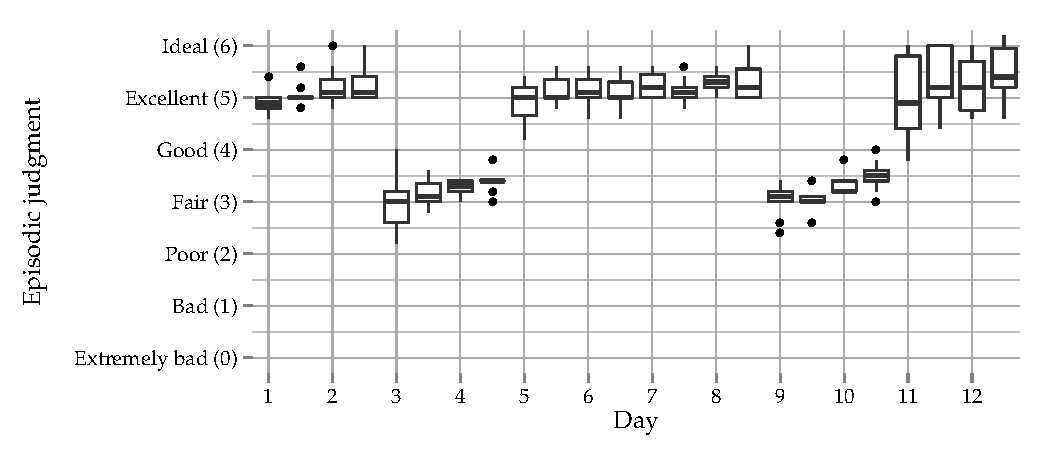
\includegraphics[width=\maxwidth]{figure/plotMOLLER-1} 

\end{knitrout}
	\caption[\citet{moller_single-call_2011}: box plot of episodic judgments for condition~4]{Box plot of episodic judgments for condition~4 of \citet{moller_single-call_2011} (own illustration).}
	\label{img:state:MOLLERboxplot}
\end{figure}

\begin{table}[b]
	\centering
	\caption[\citet{moller_single-call_2011}: episodic judgments and multi\-/episodic judgments]{Episodic judgments and multi\-/episodic judgments by \citet{moller_single-call_2011}. Reported as \ac{MOS} with standard deviation in brackets.}
	\label{tab:state:MOLLERepisodic}
	\begin{tabular}{c||c|c|c||c|c|c}
	\multirow{2}{*}{\rotatebox{90}{Cond.}} & \multicolumn{3}{c||}{Episodic judgments} &  \multicolumn{3}{c}{Multi-episodic judgments} \\
	  & \ac{HP}	& \ac{MP} & \ac{LP} & 2nd	day & 7th day & 12th day \\
	\midrule
	1 			& 5.5 (0.7) & - & - & 5.4 (0.3) & 5.3 (0.5) & 5.7 (0.8) \\
	\hline
	2 			& 5.2 (0.8) & - & 3.9 (1.1) & 5.3 (0.7) & 5.1 (0.7) & 5.5 (0.5) \\
	\hline
	3 			& 4.9 (1.0) & - & 4.0 (1.0) & 5.1 (0.6) & 4.8 (0.6) & 4.9 (0.8) \\
	\hline
	4 			& 4.9 (0.8) & - & 3.7 (0.8) & 5.1 (0.3) & 4.7 (0.2) & 4.8 (0.6) \\
	\hline
	5 			& -	& 4.8 (0.8) & 3.9 (1.1) & 4.9 (0.3) & 4.8 (0.4) & 4.9 (0.6) \\
	\end{tabular}
\end{table}

\subparagraph*{Episodic Judgments}
For all conditions, the episodic judgments reflect the applied episodic performance level, \ie, \ac{HP} and \ac{MP} are judged to be better than \ac{LP}.
It can thus be concluded that the technical setup worked as desired.
%Condition 5 is evaluated alone as the absence of \ac{HP} might affect episodic and multi\-/episodic judgments
However, comparing the episodic judgments for \ac{HP} episodes between the conditions~1..4 shows significant differences ($H(3)=69.2911$, $p<0.001$).
A post-hoc test (pairwise Wilcoxon rank-sum test with Holms' correction) shows that the episodic judgments for \ac{HP} are not significantly different between condition~3 and condition~4 ($p=0.137$), but all other conditions are significantly different to each other ($p\leq0.04$). %wilcox.pairwise.print(QU~condition, "MOELLER", "HP", c("S1", "S2", "S3", "S5"))
Episodic judgments of \ac{LP} are not significantly different between conditions~2..4 ($H(2)=4.8033$, $p=0.0906$).
The observed difference for episodic judgments of \ac{HP} are relatively small and are likely an artifact of the between-subject design.

For condition~2..4, a significant difference between the two performance levels is observed ($W=90159.00$, $p<0.001$).
It must be noted that although \ac{HP} and \ac{LP} were judged to be different, \ac{LP} was still judged approximately as \emph{fair}.
It thus does not seem to be perceived as a \emph{severe} degradation.
With regard to condition~5, the episodic judgments of \ac{LP} episodes are close to conditions~2..4.
In fact, \ac{MP} judgments are only slightly lower than \ac{HP} judgments for conditions~1..4.
As \ac{MP} and \ac{HP} were not presented together, this indicates that either the scale was used differently between conditions or that both performance levels were perceived as similar.

The results show that the defined-use method could be applied successfully, as episodic judgments could be taken reliably even in a field experiment.
\citet{moller_single-call_2011} noted that episodic judgments of \ac{HP} episodes have a tendency to slowly increase over the usage period.
Here, an increase of \unit[0.3]{pt} of \ac{MOS} is reported over all five conditions.
In addition, it is reported that the judgments of \ac{HP} episodes that follow \ac{LP} episodes seem to be negatively affected by the preceding \ac{LP} episodes.
\citet{moller_single-call_2011} suggested a recovery period of up to two episodes for episodic judgments.
A statistical analysis is omitted due to the relative small (potential) difference between episodic judgments, the high standard deviation, and the small number of participants.

\subparagraph*{Multi-episodic Judgments}
With regard to multi\-/episodic judgments, the result of this experiment are limited.
Here, the multi\-/episodic judgments are rather close, ranging only from 4.7 (0.2) to 5.7 (0.8).
A significant difference between the multi\-/episodic judgments per condition is only found for condition~4 ($H(2)=8.4114$, $p=0.0149$).
In all other conditions, no significant difference is observed.
For condition~4, a post-hoc test (pairwise Wilcoxon rank-sum test with Holms' correction) shows that the multi\-/episodic judgment after the 2nd~day is significantly different from the judgment after the 7th~day ($p=0.003$).
However, the judgment after the 2nd~day and the 7th~day are not significantly different from the judgment after the 12th~day (each $p=0.450$).
In fact, an absolute comparison with regard to multi\-/episodic judgments between the five conditions conducted must be omitted due to the observed differences for episodic judgments between the conditions, \ie, an artifact that might be attributed to the between-subject design.
It must thus be concluded that only condition~4 resulted in an observable, although rather small, effect on multi\-/episodic judgments due to the presentation of the 3rd and 4th~day in \ac{LP}.

%With regard to condition~5 an interesting observation can be made.
%It is notable that multi\-/episodic judgments for condition~5 were rather close to the other conditions.
%This also indicates that \ac{MP} and \ac{HP} did not affect multi\-/episodic judgments.

%kruskal(IQU~condition, "MOELLER", c("HP", "LP"), c("S1", "S2", "S3", "S4", "S5"), "4") %N
%kruskal(IQU~condition, "MOELLER", c("HP", "LP"), c("S1", "S2", "S3", "S4", "S5"), "14") 
%wilcox.pairwise.print(IQU~condition, "MOELLER", c("LP", "HP"), c("S1", "S2", "S3", "S5"), 14) %S2 vs. S5: 0.01
%kruskal(IQU~condition, "MOELLER", c("HP", "LP"), c("S1", "S2", "S3", "S4", "S5"), "24") %SIG
%wilcox.pairwise.print(IQU~condition, "MOELLER", c("LP", "HP"), c("S1", "S2", "S3", "S5"), 24) %N SIG
%kruskal(IQU~id, "MOELLER", c("LP", "HP"), "S1", c(4, 14, 24))
%kruskal(IQU~id, "MOELLER", c("LP", "HP"), "S2", c(4, 14, 24)) %SIG
%wilcox.pairwise.print(IQU~id, "MOELLER", c("LP", "HP"), "S2", c(4, 14, 24)) %SIG 4 vs 14: 0.003
%kruskal(IQU~id, "MOELLER", c("LP", "HP"), "S3", c(4, 14, 24))
%kruskal(IQU~id, "MOELLER", c("LP", "MP"), "S4", c(4, 14, 24))
%kruskal(IQU~id, "MOELLER", c("LP", "HP"), "S5", c(4, 14, 24))

\subparagraph{Discussion}
\citet{moller_single-call_2011} successfully applied the defined-use method for the assessment of multi\-/episodic perceived quality in a field experiment with a usage period of 12~days.
The episodic judgments are consistent with the desired performance levels, showing that the used service could provide the performance levels in a reliable manner.
However, the multi\-/episodic judgments only provide limited insight, as the differences between conditions are rather small.
This might be due to the fact that \ac{LP} did not represent a \emph{severe} degradation, or that the number of degraded usage episodes was too low.
Alongside this, a difficulty with this experiment is that no useful details about the technical parameters were provided.
This is likely due to the use of (proprietary) technology provided by Skype.
In fact, no information about resolution, frame rate, codecs, audio signal bandwidth, echo cancellation, audio coding bandwidth, or video coding bandwidth etc. were reported.
Also, recordings or monitoring data about the actual network transmission is not available.
Another factor that might have influenced the results is the usage of a widely known service.
This might have influenced expectations, due to prior knowledge and experiences with Skype.
Furthermore, participants were allowed in this experiment to use the service for personal communication beside the defined usage pattern.
Thus, some participants might have used the service more often than others.
This might have affected their episodic judgments and also multi\-/episodic judgments.
%Selecting a two\=/party conversation (\ie, \ac{SCS}) might have been another issue.
%\acp{SCS} try to enforce a conversation flow, which is however influenced by the usage behavior of the two parties, and thus might affect the individual duration of usage episodes as reported by \citet{moller_single-call_2011}.
%This implicitly assumes a \emph{duration neglect} with regard to multi\-/episodic perceived quality.
%The effect of duration neglect, however, has not neither been proven nor disproven so far for multi\-/episodic perceived quality.
Nevertheless, \citet{moller_single-call_2011} showed the applicability of the defined-use method for investigations in field experiments.
Although participants used the service in their home environment on their own, \ie, in settings that were uncontrolled and unknown to the researchers, the episodic results show that perceived quality can be assessed successfully with this method.

\section{Conclusion}
Multi\-/episodic perceived quality has so far only received limited attention.
The work of \citet{duncanson_average_1969} and \citet{moller_single-call_2011} form a basis for the investigation of the formation process of multi\-/episodic perceived quality.
In particular, the defined-use method developed and tested by \citet{moller_single-call_2011} seems suitable for this investigation.
However, neither \citet{duncanson_average_1969} nor \citet{moller_single-call_2011} were able to investigate the formation process of multi\-/episodic perceived quality in detail.





%Starting from effects on the retrospective judgments found in assessment of general experiences (\cf{} \autoref{chap:03})
